% TikZ test for XeLaTeX engine
\documentclass{article}
\usepackage{fontspec}
\usepackage{tikz}

\setmainfont{DejaVu Serif}
\setsansfont{DejaVu Sans}

\title{TikZ Test (XeLaTeX)}
\author{MiKTeX Test Suite}
\date{\today}

\begin{document}

\maketitle

\section{Simple Shapes}
This document tests TikZ drawings with XeLaTeX.

\begin{center}
\begin{tikzpicture}
  \draw (0,0) circle (1cm);
  \draw (2,0) rectangle (3,1);
  \draw (4,0) -- (5,1);
  \draw (6,0.5) ellipse (0.5cm and 1cm);
\end{tikzpicture}
\end{center}

\section{Colored Shapes}
\begin{center}
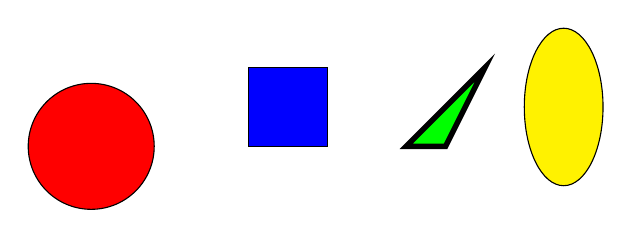
\begin{tikzpicture}
  \draw[fill=red] (0,0) circle (0.8cm);
  \draw[fill=blue] (2,0) rectangle (3,1);
  \draw[fill=green, draw=black, line width=2pt] (4,0) -- (5,1) -- (4.5,0) -- cycle;
  \draw[fill=yellow] (6,0.5) ellipse (0.5cm and 1cm);
\end{tikzpicture}
\end{center}

\section{Coordinate System}
\begin{center}
\begin{tikzpicture}[scale=1.5]
  \draw[->] (-0.5,0) -- (2.5,0) node[right] {$x$};
  \draw[->] (0,-0.5) -- (0,2.5) node[above] {$y$};
  \draw[red,thick] plot[domain=0:2] (\x, \x*\x);
  \draw[blue,thick] plot[domain=0:2] (\x, 2-\x);
\end{tikzpicture}
\end{center}

\section{Unicode Labels}
\begin{center}
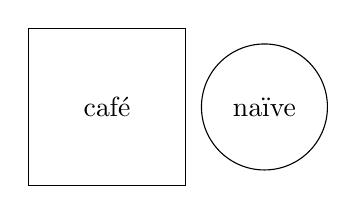
\begin{tikzpicture}
  \draw (0,0) rectangle (2,2) node[midway] {café};
  \draw (3,1) circle (0.8) node {naïve};
\end{tikzpicture}
\end{center}

\section{Conclusion}
TikZ diagrams render successfully with XeLaTeX and Unicode.

\end{document}
